\section{Auswertung}
\label{sec:Auswertung}

\subsection{Bestimmung von $U_0$ und $R_i$ der Monozelle}

Es wird die Klemmspannung $U_k$ in Abhängigkeit des Stromes $I$ gemessen. 
Die aufgenommenen Werte sind in Tabelle \ref{tab:Monozelle} aufgeführt. 

\begin{table}
\centering
\caption{Spannungs- und Stromwerte der Monozelle}
\label{tab:Monozelle}
\sisetup{table-format=2.1}
\begin{tabular}{c c}
\toprule
$U_k \,/\, \si{\volt}$ & $I \,/\, \si{\milli\ampere}$\\
\midrule
1.550 &  25.0\\
1.525 &  27.5\\
1.500 &  31.0\\
1.450 &  38.0\\
1.425 &  46.0\\
1.400 &  49.5\\
1.350 &  57.0\\
1.300 &  61.5\\
1.250 &  77.5\\
1.200 &  85.0\\
1.100 & 110.0\\
0.700 & 175.0\\
0.450 & 215.0\\
0.400 & 225.0\\
\bottomrule
\end{tabular}
\end{table}

Es wird eine lineare Regression durchgeführt, um die Leerlaufspannung $U_0$ 
und den Innenwiderstand $R_i$ zu berechnen. Hierfür verwenden wir Python mit 
der Bibliothek Numpy.
Es ergibt sich die in Abbildung \ref{fig:plot1} dargestellte Ausgleichsgerade:

\begin{equation}
U(I) = m\cdot I + b 
\label{eqn:Gerade}
\end{equation}

Mit den Parametern

\begin{align*}
m &= \SI{-5.655+-0.0776}{\volt\per\ampere}\\
b &= \SI{1.680+-0.0085}{\volt}
\end{align*}

\begin{figure}
  \centering
  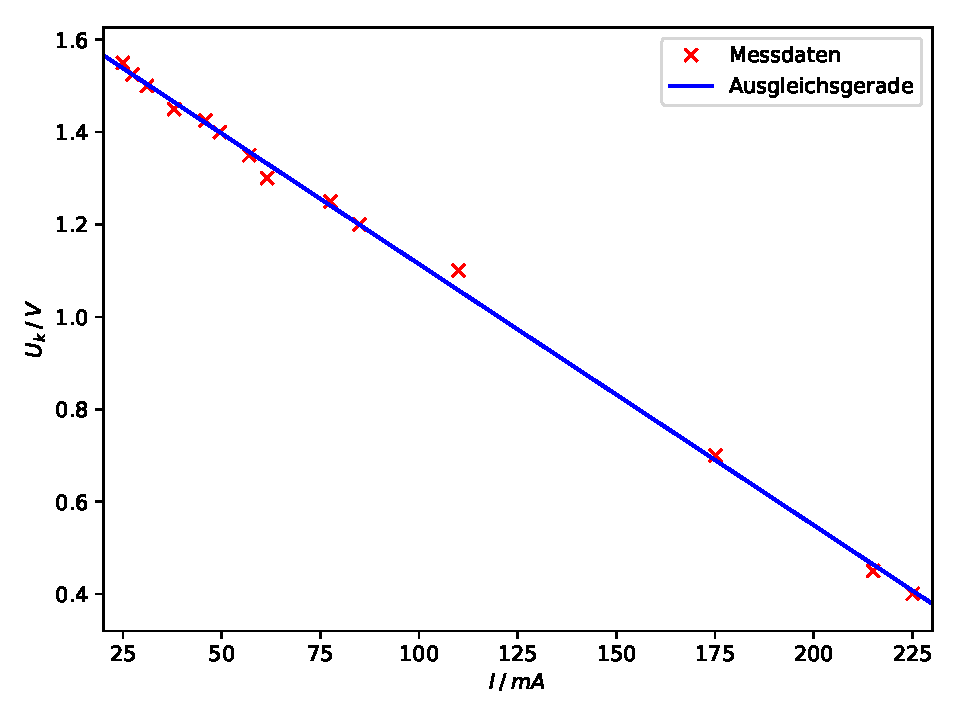
\includegraphics[scale=0.75]{content/plot1.pdf}
  \caption{Strom- und Spannungsmesswerte einer Monozelle mit Regression}
  \label{fig:plot1}
\end{figure}

Durch Vergleich mit (\ref{eqn:Maschenregel}) ergeben sich somit 
die gesuchten Größen zu: 

\begin{align*}
R_i &= \SI{5.655+-0.0776}{\ohm}\\
U_0 &= \SI{1.680+-0.0085}{\volt}
\end{align*}

Man erkennt, dass der Wert für die Leerlaufspannung annäherend mit dem zuvor
gemessenen Wert $U_0 = \SI{1.65}{\volt}$ übereinstimmt. Die Abweichung entsteht
durch einen systematischen Fehler, der durch den endlichen Innenwiderstand des
Voltmeters entsteht.
Dazu wird das Ohmsche Gesetz auf $R_i$ und $R_v$ angewendet, nach $I$ umgestellt
und in \ref{eqn:Maschenregel} angewendet.

\begin{align*}
&\quad U_k = U_0 - \frac{U_0}{R_i+R_v}\cdot R_i\\
&\Leftrightarrow U_0 = U_k\cdot (1 + \frac{R_i}{R_v})
\end{align*}

Der systematische Fehler beträgt somit:

\begin{equation}
\Delta U = U_k\cdot \frac{R_i}{R_v}
\end{equation}

Mit den Werten $U_k = \SI{1.65}{\volt}$, $R_i = \SI{5.655}{\ohm}$ und 
$R_v = \SI{10}{\mega\ohm}$ ergibt sich der Wert $\Delta U = \SI{933}{\nano\volt}$.
Dies ist im Vergleich zur gemessenen Spannung verschwindend gering.

\subsection{Bestimmung von $U_0$ und $R_i$ der Monozelle mit Gegenspannung}

Nun wird die gleiche Messung mit einer angelegten Gegenspannung durchgeführt.
Die gemessenen Werte sind in Tabelle \ref{tab:Gegen} aufgeführt.

\begin{table}
  \centering
  \caption{Spannungs- und Stromwerte der Monozelle unter Gegenspannung}
  \label{tab:Gegen}
  \sisetup{table-format=2.1}
  \begin{tabular}{c c}
    \toprule
     $U_k \,/\, \si{\volt}$ & $I \,/\, \si{\milli\ampere}$\\
    \midrule
      1.900 &  40.0\\
      1.925 &  42.0\\
      1.950 &  45.5\\
      1.975 &  52.5\\
      2.000 &  55.5\\
      2.050 &  65.0\\
      2.100 &  73.0\\
      2.150 &  82.5\\
      2.200 &  90.0\\
      2.250 & 101.0\\
      2.300 & 105.0\\
      2.400 & 120.0\\
      2.500 & 140.0\\
      2.700 & 170.0\\
      3.000 & 220.0\\
    \bottomrule
  \end{tabular}
\end{table}

Auch hier wird eine lineare Regression mittels Phyton und Numpy durchgeführt.
Das Resultat ist in Abbildung \ref{fig:plot2} zu sehen.

\begin{figure}
  \centering
  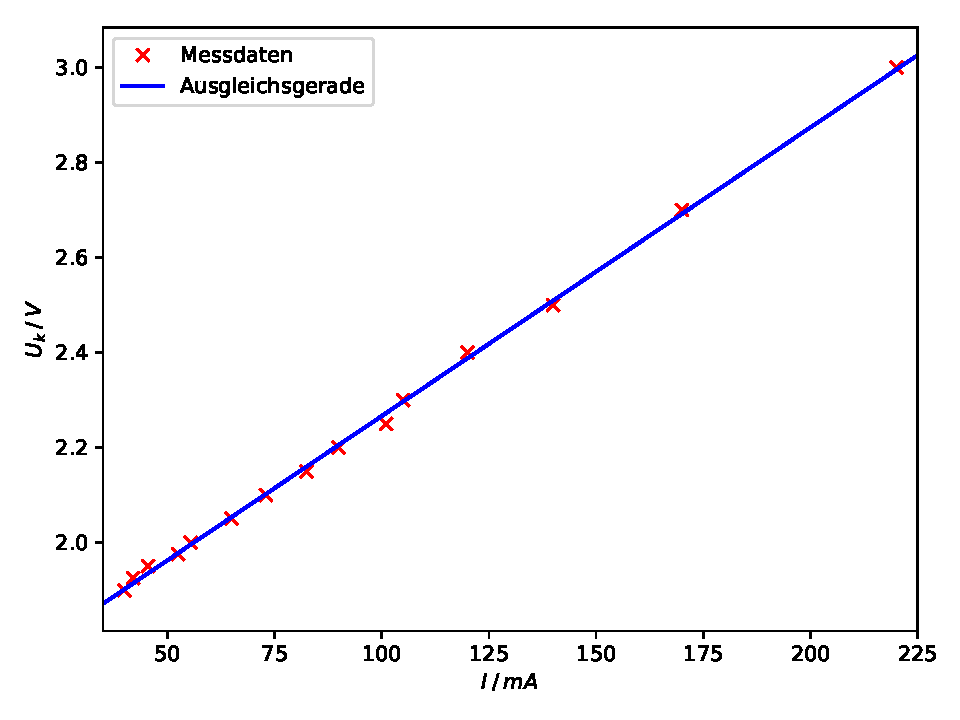
\includegraphics[scale=0.75]{content/plot2.pdf}
  \caption{Strom - und Spannungsmesswerte einer Monozelle bei Verwendung einer Gegenspannung}
  \label{fig:plot2}
\end{figure}

Die Ausgleichsgerade hat eine positive Steigung. Dies liegt daran, dass 
der Strom in entgegengesetzter Richtung durch die Monozelle fließt. 
Die Geradengleichung lautet gemäß (\ref{eqn:Gerade}). Dabei ergeben sich diesmal 
die Parameter: 

\begin{align*}
m &= \SI{6.0770+-0.0576}{\volt\per\ampere}\\
b &= \SI{1.6587+-0.0061}{\volt}
\end{align*}

Damit ergibt sich die gesuchten Werte analog, wobei der Strom mit
einem umgekehrten Vorzeichen versehen wird:

\begin{align*}
R_i &= \SI{6.0770+-0.0576}{\ohm}\\
U_0 &= \SI{1.6587+-0.0061}{\volt}
\end{align*}

Es ist zu erkennen, dass der errechnete Wert für die Leerlaufspannung
und der gemessene bei diesem Aufbau noch besser übereinstimmen.

\subsection{Bestimmung von $U_0$ und $R_i$ des Rechteckausgangs
            eines RC-Generators}

Es werden $U_k$ und $I$ von einer Rechteckspannung gemessen. Die Messwerte
sind in Tabelle \ref{tab:Rechteck} aufgeführt.

\begin{table}
   \centering
   \caption{Spannungs- und Stromwerte der Rechteckspannung}
   \label{tab:Rechteck}
   \sisetup{table-format=2.1}
   \begin{tabular}{c c}
      \toprule
       $U_k \,/\, \si{\volt}$ & $I \,/\, \si{\milli\ampere}$\\
      \midrule
        0.54 & 2.15\\
        0.52 & 2.50\\
        0.50 & 2.85\\
        0.48 & 3.25\\ 
        0.46 & 3.65\\
        0.42 & 4.55\\
        0.38 & 5.20\\
        0.35 & 5.80\\
        0.30 & 6.75\\
        0.25 & 7.7\\
        0.20 & 8.55\\
      \bottomrule
   \end{tabular}
\end{table}

Auch hier wird eine lineare Regression durchgeführt mittels Python 
und Numpy. Die Messwerte und Ausgleichsgerade sind in Abbildung \ref{fig:plot3}
zu sehen.

\begin{figure}
  \centering
  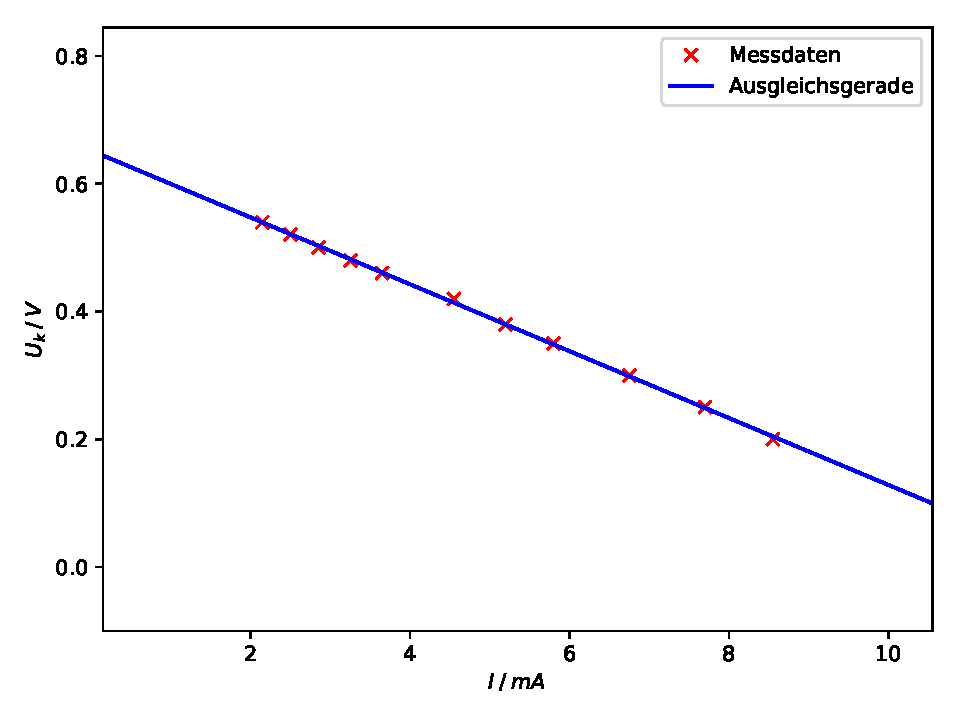
\includegraphics[scale=0.75]{content/plot3.pdf}
  \caption{Strom- und Spannungsmesswerte einer Rechteckspannung}
  \label{fig:plot3}
\end{figure}

Die Parameter ergeben sich diesmal gemäß (\ref{eqn:Gerade}) zu: 

\begin{align*}
m &= \SI{-52.350+-0.4829}{\volt\per\ampere}\\
b &= \SI{0.652+-0.0025}{\volt}
\end{align*}

Somit ergeben sich gemäß (\ref{eqn:Maschenregel}) folgende Werte:

\begin{align*}
R_i &= \SI{52.350+-0.4829}{\ohm}\\
U_0 &= \SI{0.652+-0.0025}{\volt}
\end{align*}

\subsection{Bestimmung von $U_0$ und $R_i$ des Sinusausgangs eines RC-Generators}

Es werden $U_k$ und $I$ von einer Sinusspannung gemessen. Die Messwerte
sind in Tabelle \ref{tab:Sinus} aufgeführt.

\begin{table}
   \centering
   \caption{Spannungs- und Stromwerte der Sinusspannung}
   \label{tab:Sinus}
   \sisetup{table-format=2.1}
   \begin{tabular}{c c}
     \toprule
      $U_k \,/\, \si{\volt}$ & $I \,/\, \si{\milli\ampere}$\\
     \midrule
       2.100 & 0.355\\
       2.000 & 0.600\\
       1.900 & 0.650\\
       1.800 & 0.850\\
       1.750 & 0.950\\
       1.700 & 1.050\\
       1.650 & 1.100\\
       1.600 & 1.200\\
       1.550 & 1.275\\
       1.500 & 1.350\\
       1.450 & 1.425\\
       1.400 & 1.500\\
       1.375 & 1.575\\
       1.300 & 1.650\\
       1.250 & 1.725\\
       1.000 & 2.125\\
       0.750 & 2.550\\
     \bottomrule
   \end{tabular}
 \end{table}

Auch hier wird eine lineare Regression durchgeführt mittels Python 
und Numpy. Die Messwerte und Ausgleichsgerade sind in Abbildung \ref{fig:plot4}
zu sehen.

\begin{figure}
  \centering
  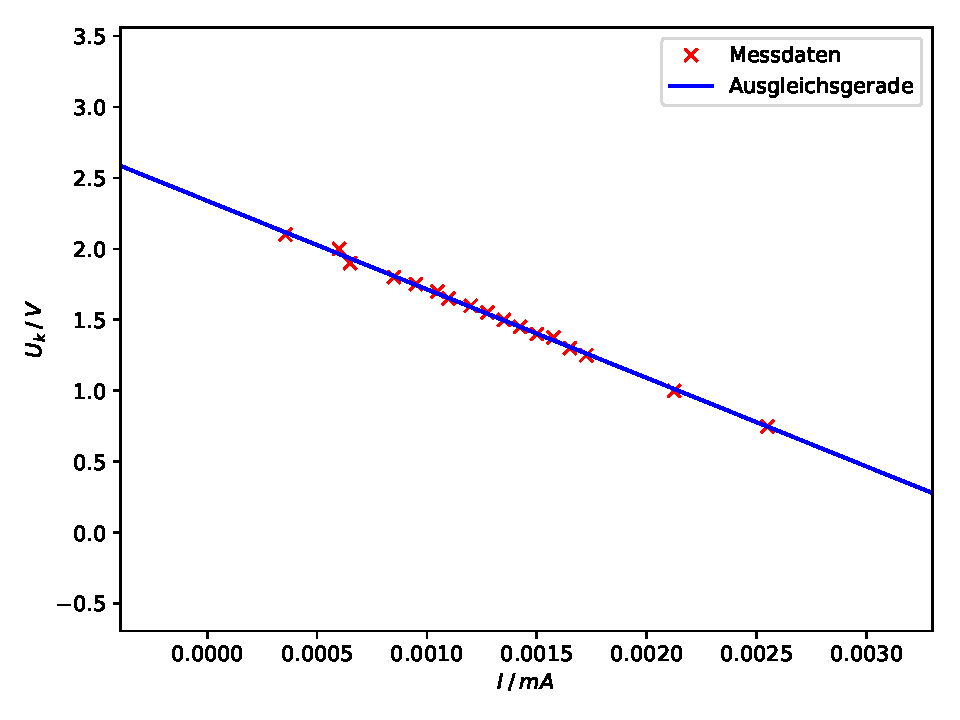
\includegraphics[scale=0.75]{content/plot4.pdf}
  \caption{Strom- und Spannungsmesswerte einer Sinusspannung}
  \label{fig:plot4}
\end{figure}

Die Parameter ergeben sich diesmal gemäß (\ref{eqn:Gerade}) zu: 

\begin{align*}
m &= \SI{624.117+-7.8725}{\volt\per\ampere}\\
b &= \SI{2.339+-0.011}{\volt}
\end{align*}

Somit ergeben sich gemäß (\ref{eqn:Maschenregel}) folgende Werte:

\begin{align*}
R_i &= \SI{624.117+-7.8725}{\ohm}\\
U_0 &= \SI{2.339+-0.011}{\volt}
\end{align*}

\subsection{Systematischer Fehler eines in Reihe geschalteten Voltmeters}

Nun soll die Schaltung, die in Abbildung \ref{fig:Ersatz} dargestellt ist, 
so variiert werden, dass das Voltmeter in Reihe geschaltet wird.
Dabei verändert sich die Klemmspannung $U_k$ nach der 2. Kirchhoffschen Regel:

\begin{align*}
U_k &= U_{am} + U_{vm} + U_{Ra}\\
U_k &= R_{am}\cdot I + R_{vm}\cdot I + R_a\cdot I  
\end{align*}

Dabei bezeichnet $U_{am}$ die Spannung, die über das Amperemeter,
$U_{vm}$, die über das Voltmeter und $U_{Ra}$, die über den Widerstand
abfällt.

Entgegen unser vorherigen Betrachtung kann hier $U_0$ nicht als $U_k$
angenommen werden. Dies liegt daran, dass das Voltmeter mit einem 
hochohmigen Innenwiderstand behaftet ist.

\subsection{Leistungskurve}

Aus den Messwerten in Kapitel 4.1 werden der Belastungswiderstand und 
die im Widerstand umgesetzte Leistung berechnet. Die Werte sind in 
Tabelle \ref{tab:Leistung} aufgetragen.

\begin{table}
   \centering
   \caption{Errechnete Leistungswerte}
   \label{tab:Leistung}
   \sisetup{table-format=2.1}
   \begin{tabular}{c c c c}
     \toprule
      $U_k \,/\, \si{\volt}$ & $I \,/\, \si{\milli\ampere}$ & $R_a \,/\, \si{\ohm}$ & $P \,/\, \si{\watt}$\\
     \midrule
      1.550 &  25.0 & 62.00 & 0.039\\
      1.525 &  27.5 & 55.45 & 0.042\\
      1.500 &  31.0 & 48.39 & 0.047\\
      1.450 &  38.0 & 38.16 & 0.055\\
      1.425 &  46.0 & 30.98 & 0.066\\
      1.400 &  49.5 & 28.28 & 0.069\\
      1.350 &  57.0 & 23.68 & 0.077\\
      1.300 &  61.5 & 21.14 & 0.080\\
      1.250 &  77.5 & 16.13 & 0.097\\
      1.200 &  85.0 & 14.12 & 0.102\\
      1.100 & 110.0 & 10.00 & 0.121\\
      0.700 & 175.0 &  4.00 & 0.123\\
      0.450 & 215.0 &  2.09 & 0.096\\
      0.400 & 225.0 &  1.77 & 0.890\\
     \bottomrule
   \end{tabular}
 \end{table}

Nach (\ref{eqn:Leistungsfunktion}) wird nun die Leistung $P$ gegen den
Belastungswiderstand $R_a$ aufgetragen. Die Theoriekurve ergibt sich aus 
den Werten:

\begin{align*}
R_i &= \SI{5.66}{\ohm}\\
U_0 &= \SI{1.68}{\volt}
\end{align*}

Sowohl die Kurve als auch die Messwerte sind in Abbildung \ref{fig:plot5}
dargestellt. 

\begin{figure}
  \centering
  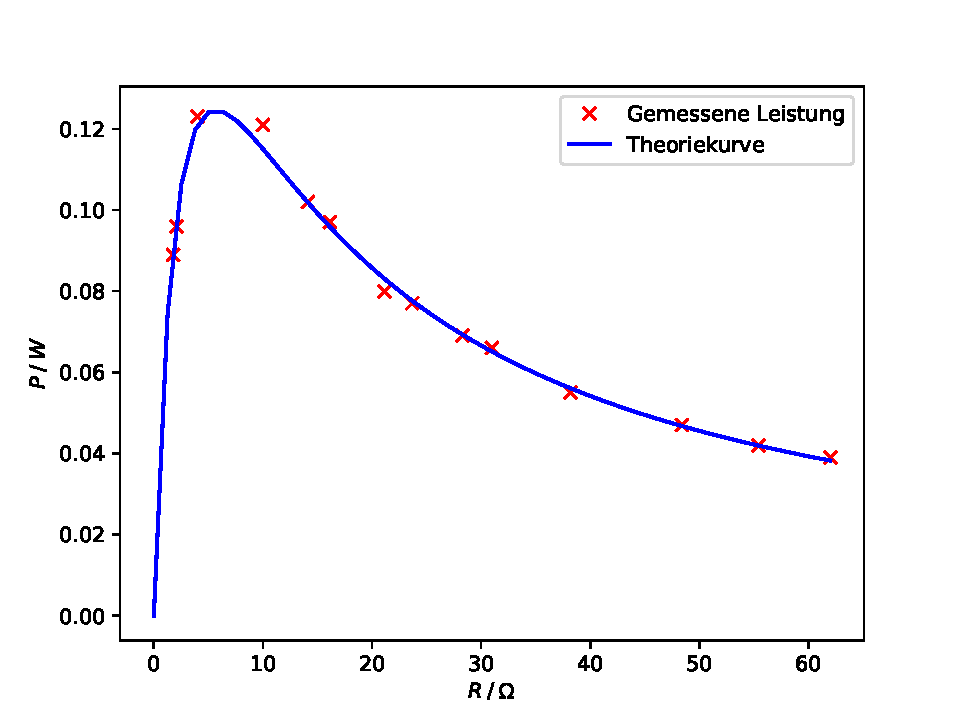
\includegraphics[scale=0.75]{content/plot5.pdf}
  \caption{Umgesetzte Leistung aufgetragen gegen den Lastwiderstand}
  \label{fig:plot5}
\end{figure}

Es ist zu erkennen, dass die Theoriekurve sehr gut zu den Messdaten passt 
und diese nur geringfügig abweichen. Es sind neben Messungenauigkeiten
keine systematischen Fehler zu erkennen. 